\providecommand{\main}{../../../..}
\documentclass[\main/dresen_thesis.tex]{subfiles}

\begin{document}
  \label{sec:colloidalCrystals:nanoparticle:xrd}
  \begin{figure}[tb]
    \centering
    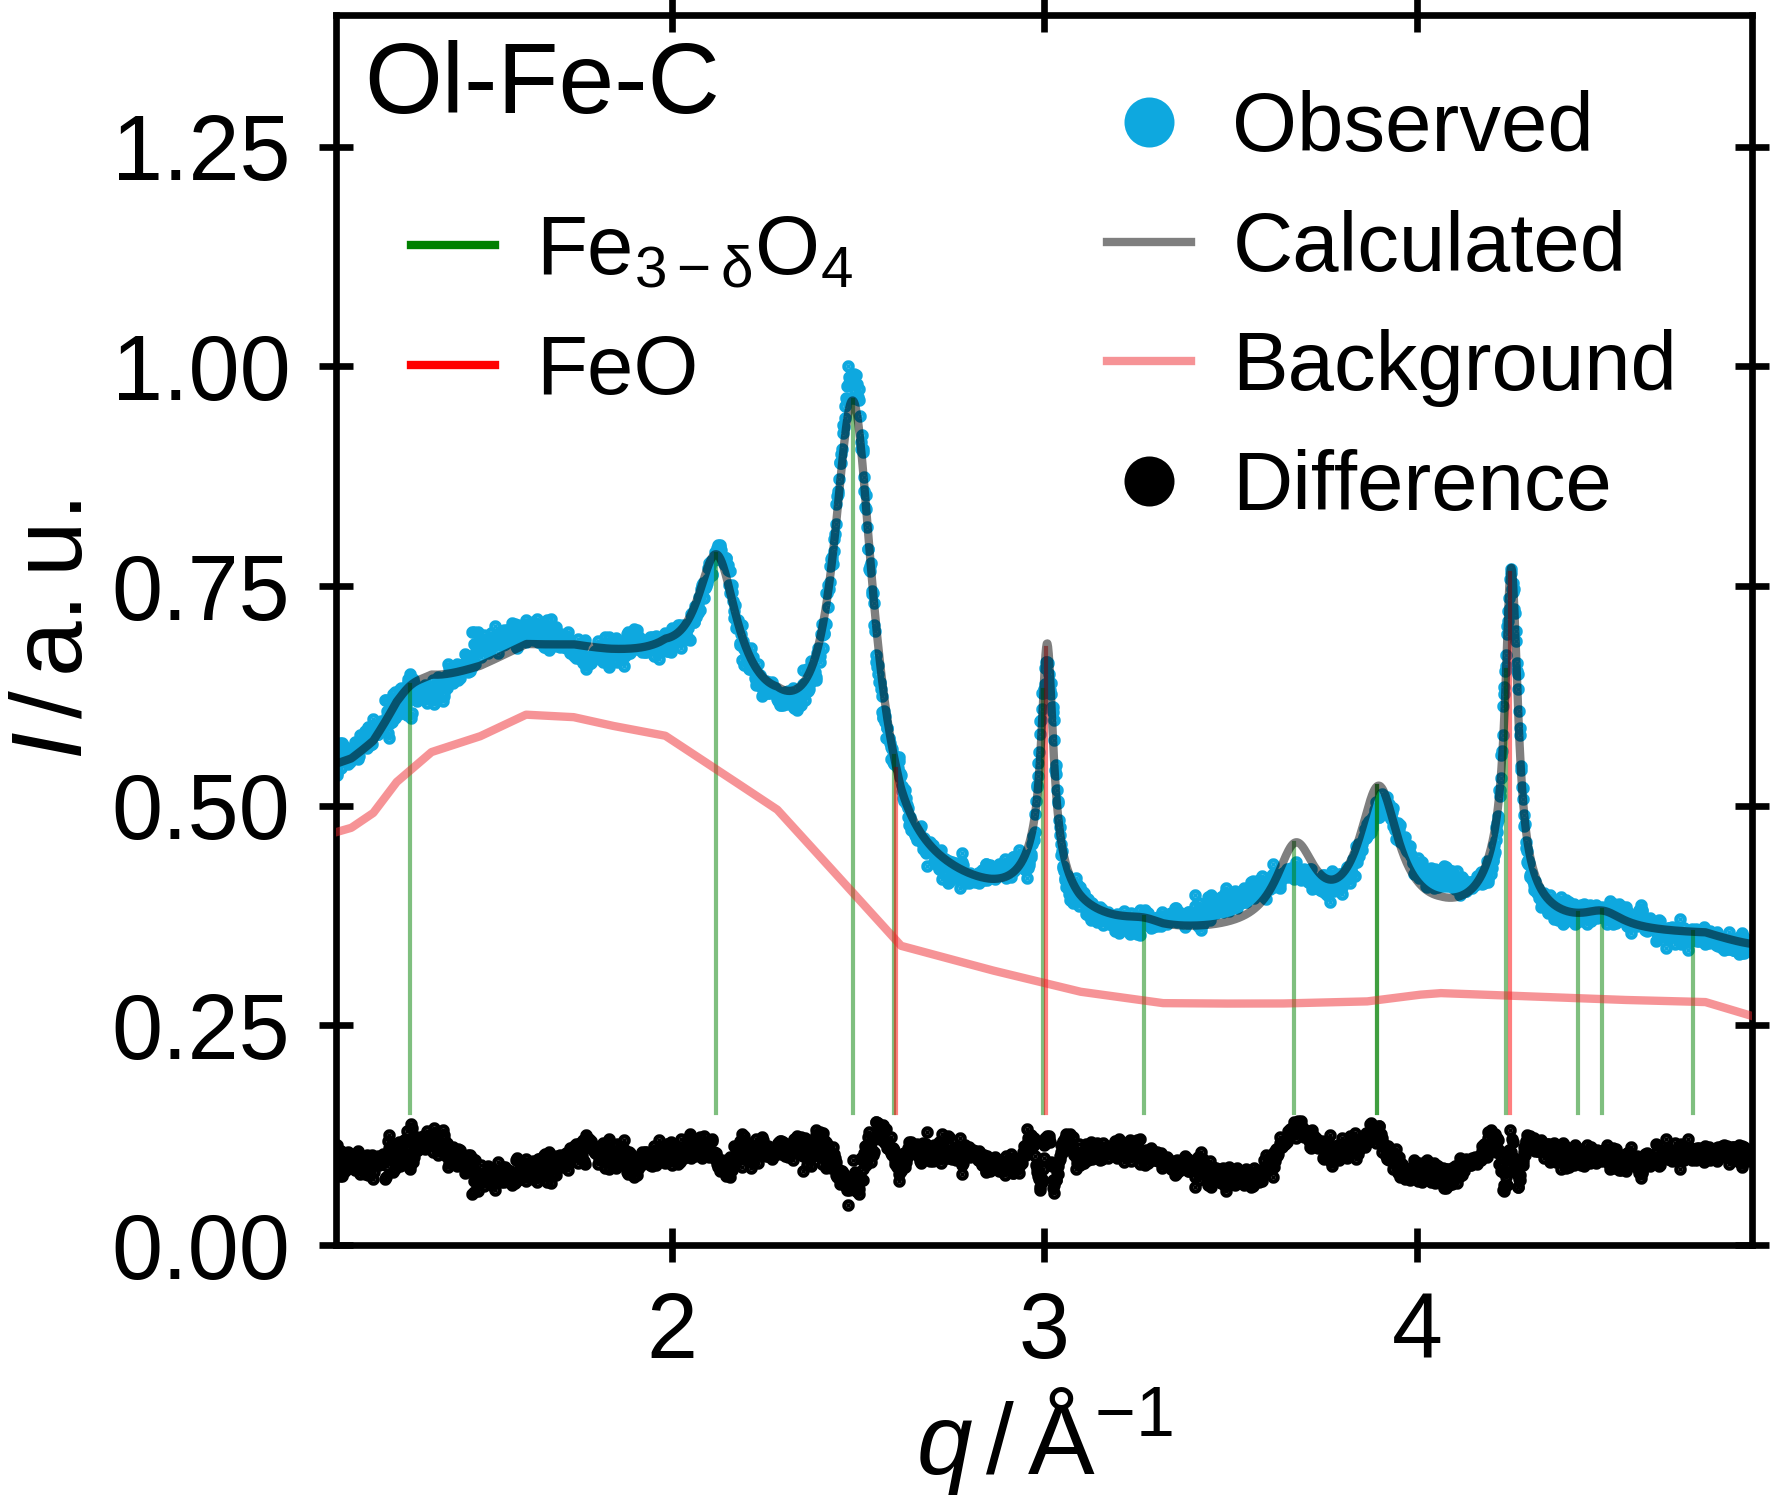
\includegraphics{colloidalCrystals_XRD_Fe3O4WustiteFit_Ol_Fe_C}
    \caption{\label{fig:colloidalCrystals:nanoparticle:xrd}X-ray diffraction of Ol-Fe-C with a LeBail refinement of a combination of an inverse spinell and a w\"ustite phase. The manually estimated background is shown as red line.}
  \end{figure}

  The X-ray diffraction in \reffig{fig:colloidalCrystals:nanoparticle:xrd} for Ol-Fe-C shows multiple reflections, which can be associated with an inverse spinell structure.
  The diffractogram is similar to the one measured for iron oxide nanospheres from oleates, which was discussed in \refsec{sec:looselyPackedNS:nanoparticle:xrd} and the same discussion can be done.
  Similarly, two phases are necessary for a proper description, as a closer inspection shows that the reflections around $3 \unit{\angstrom}$ and $4.2 \unit{\angstrom}$ have a lower peak width than the remaining reflections.
  By including a w\"ustite phase, the LeBail refinement yields a close match to the experimental data as shown in \reffig{fig:colloidalCrystals:nanoparticle:xrd}.

  The determined lattice constants $a$ of the two phases, and the Lorentzian isotropic size parameter $Y$ are tabulated together with the determined crystallite sizes $L$ in \reftab{tab:colloidalCrystals:nanoparticle:discussion:xrdLeBail}.

  \begin{table}[ht]
    \centering
    \caption{\label{tab:colloidalCrystals:nanoparticle:discussion:xrdLeBail}Refined parameters of the LeBail fit of Ol-Fe-C. Tabulated are the parameters of the lattice constants $a$, the Lorentzian isotropic size parameter $Y$ and the calculated crystallite size $L$ for both phases. Also given are the used wavelength $\lambda$, the figure of merit $\chi^2$ and the agreement factors $R$.}
    \begin{tabular}{ l | l }
      \hline
      \rule{0pt}{2ex} \textbf{XRD} & \textbf{Ol-Fe-C}\\
      \hline
      \hline
      \rule{0pt}{2ex}space group & $Fd\bar{3}m$ (No. 227) + $Fm\bar{3}m$ (No. 225)\\
      \hline
      \rule{0pt}{2ex} $a_\mathrm{inv. spinell} \,/ \unit{\angstrom}$         &  $8.3841(3)$  \\
      \rule{0pt}{2ex} $Y_\mathrm{inv. spinell} \,/ \unit{^\circ}$            &  $1.776 (6)$   \\
      \rule{0pt}{2ex} $a_\textsf{w\"ustite}     \,/ \unit{\angstrom}$        &  $4.1809(1)$  \\
      \rule{0pt}{2ex} $Y_\textsf{w\"ustite}     \,/ \unit{^\circ}$           &  $0.440(3)$   \\
      \hline
      \rule{0pt}{2ex} $L_\mathrm{inv. spinell} \,/ \unit{nm}$                &  $3.164(2)$ \\
      \rule{0pt}{2ex} $L_\textsf{w\"ustite}      \,/ \unit{nm}$              &  $12.785(4)$ \\
      \hline
      \rule{0pt}{2ex} $\lambda \,/ \unit{\angstrom}$                         &  $1.54056$\\
      \hline
      \rule{0pt}{2ex} $\chi^2$                                               &  $1.70$ \\
      \rule{0pt}{2ex} $R_p$                                                  &  $1.52$ \\
      \rule{0pt}{2ex} $R_{wp}$                                               &  $1.94$ \\
      \rule{0pt}{2ex} $R_{exp}$                                              &  $1.48$ \\
      \rule{0pt}{2ex} $R_{f, \, \mathrm{inv. spinell}}$                      &  $0.10$ \\
      \rule{0pt}{2ex} $R_{f, \, \text{w\"ustite}}$                           &  $0.15$ \\
      \hline
    \end{tabular}
  \end{table}

  \paragraphNewLine{Lattice constant}
    The lattice constant of the two phases of Ol-Fe-C are $8.3841(3) \unit{\angstrom}$ for the inverse spinell phase and $4.1809(1) \unit{\angstrom}$ for the w\"ustite phase.
    In comparison to the bulk values of magnetite/maghemite ($a_\mathrm{magnetite} \eq 8.396 \unit{\angstrom}$, $a_\mathrm{maghemite} \eq 8.340 \unit{\angstrom}$) \cite{Cornell_2003_Their} and w\"ustite ($a_\mathrm{FeO} \eq 4.33 \unit{\angstrom}$ \cite{Hentschel_1970_Stoich}), a reduced lattice constant for the w\"ustite phase and a lattice constant close to magnetite for the inverse spinell phase is observed.
    This is analogue to the observations that were made for the iron oxide nanospheres in \refsec{sec:looselyPackedNS:nanoparticle:xrd}.

    Thus it can be assumed from the lattice constants that the phase of the shell is close to magnetite, and that the reduced lattice constant of the w\"ustite core stems from a high pressure that the shell exerts on the core due to the lattice mismatch.

  \paragraphNewLine{Crystallite Size}
    The crystallite sizes obtained from the Lorentzian isotropic size parameters $Y$, are $12.785(4) \unit{nm}$ for the w\"ustite core and $3.164(2) \unit{nm}$ for the inverse spinell phase.
    The separate crystallite sizes fit into the mean nanocube edge length determined by TEM ($13.42(9) \unit{nm}$). 
    Due to the complex core-shell and cube structure, it is however not straight-forward to sum the crystallite size for direct comparison of the particle size.
    The relatively small inverse spinell phase size suggests that the particles have not undergone a strong oxidation process and are still to a large fraction in a w\"ustite phase.

\end{document}